\begin{figure}[htbp]
\centering
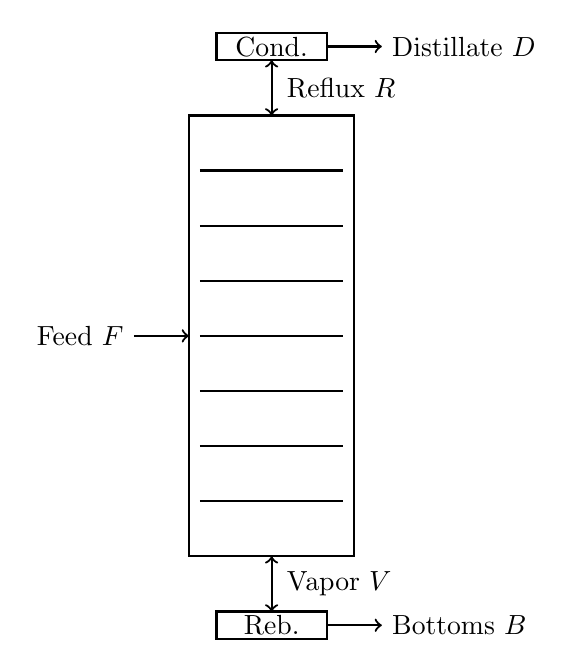
\begin{tikzpicture}[scale=0.7]
    % Column
    \draw[thick] (0,0) -- (0,8) -- (3,8) -- (3,0) -- cycle;

    % Trays
    \foreach \y in {1,2,...,7} {
        \draw[thick] (0.2,\y) -- (2.8,\y);
    }

    % Feed
    \draw[->, thick] (-1,4) -- (0,4) node[left, pos=0] {Feed $F$};

    % Overhead
    \draw[->, thick] (1.5,8) -- (1.5,9);
    \draw[thick] (0.5,9) rectangle (2.5,9.5);
    \node at (1.5,9.25) {Cond.};
    \draw[->, thick] (2.5,9.25) -- (3.5,9.25) node[right] {Distillate $D$};
    \draw[->, thick] (1.5,9) -- (1.5,8);
    \node[right] at (1.6,8.5) {Reflux $R$};

    % Bottom
    \draw[->, thick] (1.5,0) -- (1.5,-1);
    \draw[thick] (0.5,-1.5) rectangle (2.5,-1);
    \node at (1.5,-1.25) {Reb.};
    \draw[->, thick] (2.5,-1.25) -- (3.5,-1.25) node[right] {Bottoms $B$};
    \draw[->, thick] (1.5,-1) -- (1.5,0);
    \node[right] at (1.6,-0.5) {Vapor $V$};
\end{tikzpicture}
\caption{Distillation column schematic.}
\label{fig:distillation}
\end{figure}
